\section{System Architecture}
An architecture diagram is created to have a better understanding of the system architecture as well as its components.
\begin{figure}[H]
    \centering
    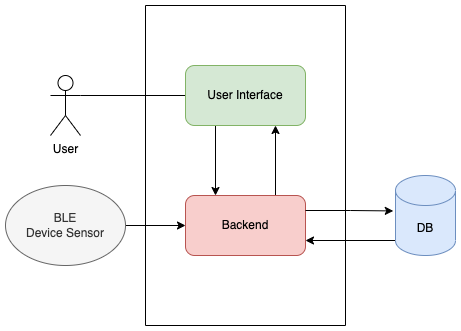
\includegraphics[width=1\textwidth]{diagrams/system-diagram.drawio.png}
    \caption{System architecture diagram}
    \label{fig:sys_diagram}
\end{figure}
The system architecture diagram illustrates the components of the systems and the interaction between the components. Within the system, there are two distinct components: the user interface and the backend which connects to a local database to store and manage data.
In addition, the device sensor is connected to the backend via bluetooth low energy and transmit the user's heart rate.